% ==================================================
% 2. Cross-method benchmark
%
% Every number here is computed from
%   benchmark/results/lmu_full_sweep_20260717/results.csv
% whose README records the command, the code revision and the machine.
% Task packet: plan/task-packets/02-benchmark.md
% ==================================================
\chapter{Cross-Method Benchmark}
\label{sec:benchmark}

\section{Setup}
\label{sec:benchmark:setup}

\begin{configtable}{Benchmark configuration}{Benchmark configuration. Provenance:
    \texttt{benchmark/results/lmu\_full\_sweep\_20260717/README.md}.}
    Games & 11 --- SOUM($n$=6,8,10) and the ML games IRIS(4), California(8), Diabetes(10),
        Adult(12), Correlated(60), Independent(60), NHANES(79), Communities(101). The ML
        grid follows Musco \& Witter. \\
    Value function & Features masked against a single baseline row (the training mean);
        \texttt{XGBRegressor}, 100 trees, depth 4. \emph{Not} any paper's value function
        --- see Chapter~\ref{sec:introduction}. \\
    Ground truth & Exact enumeration for $n \le 10$; interventional TreeSHAP against the
        same baseline row above it. \\
    Budgets & $m = c \cdot n$ for $c \in \{1,2,3,5,8,12,20,30,50,75,110,160\}$. \\
    Repeats & 10 held-out predictions per game, model fixed. Median and IQR are over
        those predictions. \\
    Methods & Every approximator registered in
        \texttt{shapiq.approximator.SV\_APPROXIMATORS} (15 registered, 14 ran). \\
    Scale & 19{,}800 cells, 143{,}980 metric rows, run on the LMU CIP cluster. \\
\end{configtable}

Two choices in that table shape everything that follows. The first is that budgets are multiples
of the number of players rather than fractions of the coalition space. A fraction of $2^n$ stops
being a runnable budget once $n$ grows --- on Independent($n$=60) even five percent of the space is
$5.8 \times 10^{16}$ evaluations --- and at the other end a budget equal to $2^n$ makes every
method exact, so ranks there record ties rather than a comparison. Multiples of $n$ are the
convention the approximator papers use, they apply to every game in the grid, and they place the
large games in the under-determined regime where the methods actually differ.

The second is that a repeat explains one held-out prediction of one fixed model. Had each repeat
retrained the model, the spread across repeats would have mixed estimator noise with model noise
and could have been read as neither: a different tree has different Shapley values, so the target
would move with the repeat. Fixing the model makes the band the spread across predictions, which
is what the approximator papers report and what a reader assumes an error band to be.

\section{Results and Discussion}
\label{sec:benchmark:results}

Averaged over all eleven games, \leverageshap{} takes the best mean rank at $3.24$, just ahead of
\oddshap{} at $3.31$, with \polyshap{} at $4.50$, OptimizedKernelSHAP at $4.69$ and RegressionMSR
at $5.46$. Reading that as a verdict would be a mistake, and the same data says why: over those
cells \oddshap{} wins outright $652$ times against \leverageshap{}'s $168$. A method that comes
first four times as often cannot also be the one that is, on average, slightly worse --- unless the
average is carried by cells in which coming first means very little.

That is what is happening. Splitting the games by dimension inverts the ordering. On the seven
small games ($n \le 12$, 840 comparison cells) \leverageshap{} leads at $3.55$, \polyshap{} follows
at $3.68$, and \oddshap{} is third at $4.51$. On the four large games ($n \ge 60$, 480 cells)
\oddshap{} leads at $1.34$, \leverageshap{} is second at $2.69$, and the best baseline,
OptimizedKernelSHAP, is far behind at $4.58$. The aggregate is not a compromise between the two
regimes; it is dominated by the first, which contributes almost twice as many cells.

The inversion is not noise but saturation. Among the small-game results $24.0\%$ are already exact
to machine precision, taking MSE below $10^{-10}$ as the threshold; among the large-game results
only $1.0\%$ are. Figure~\ref{fig:benchmark:soum} shows what that looks like: on SOUM($n$=10) every
method collapses to the numerical floor as the budget approaches $2^{10}$, and what happens to the
left of that collapse decides a rank that the collapse then erases. Where a quarter of the results
are exact, a rank is a tie-break rather than a measurement. The large games, where almost nothing
is exact, carry the comparison.

\begin{figure}[H]
    \centering
    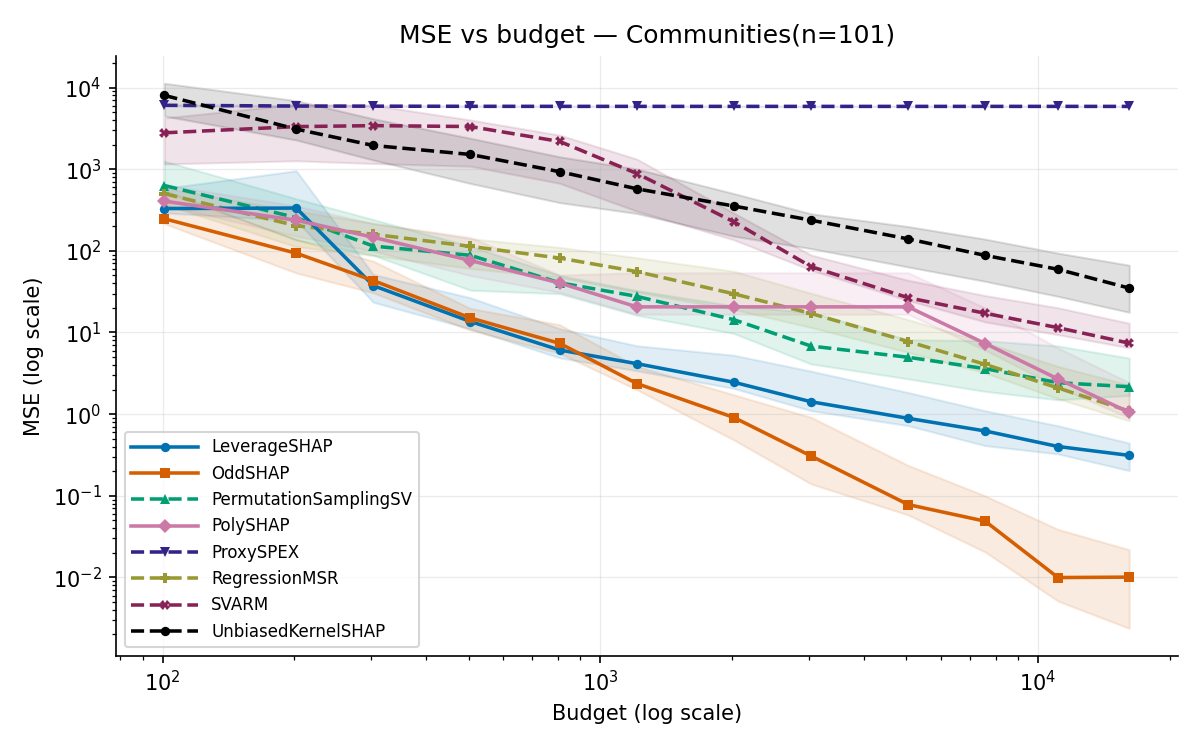
\includegraphics[width=\textwidth]{figures/bench-communities-n101.png}
    \caption[MSE against budget on Communities ($n=101$)]{MSE against budget on Communities
        ($n=101$), the largest game in the grid. Median over the ten explained predictions; the
        band is the interquartile range across them. Solid curves are the approximators added in
        this project, dashed are baselines. \oddshap{} separates from the field at roughly
        $m = 500 \approx 5d$ and ends about an order of magnitude below the runner-up.}
    \label{fig:benchmark:communities}
\end{figure}

The two regimes are not a ranking of the three methods but a division of labour between them, and
each half is what the method's own paper says it should be. Taken in turn:

\polyshap{} is second on the small games at $3.68$ and sixth on the large ones at $5.94$, the
largest swing of the three. \citet{Fumagalli.2026a} claims exactly the near half of that: in
low-dimensional settings its order-3 variant "yields the best performance" on the paper's tabular
datasets. It also states the mechanism that closes the far half --- the support is every
interaction up to a fixed order $k$, which costs $O(d^k)$ terms, so higher orders "require a
larger sampling budget". At $d = 101$ that support is unaffordable at any budget in our grid, and
the method degrades to the field. Its regime is real and it is narrow.

\leverageshap{} is the most uniform of the three: first on the small games at $3.55$ and second on
the large at $2.69$, never far from the top. \citet{Witter.2025a} makes a narrower claim than a
leaderboard position --- that leverage-score sampling "can even outperform the highly optimized
Kernel SHAP\ldots, especially for large $n$" --- and that claim is about a specific opponent, which
is in our grid. It holds, including the qualifier: \leverageshap{} leads OptimizedKernelSHAP by
$1.20$ ranks on the small games and by $1.89$ on the large ones. The advantage does not merely
survive the move to high dimension, it grows there, which is what an $O(n \log n)$ sampling
guarantee predicts against a heuristic.

\oddshap{} inverts \polyshap{}: third on the small games at $4.51$, first on the large at $1.34$,
and the gap to the runner-up is a rank and a third. On the large games its advantage also switches
on at a predictable budget. Ranking it within each budget separately gives $3.40$ at $m = d$, where
plain stratified sampling beats it; $1.35$ at $2d$; $1.30$ at $5d$; and then $1.00$, $1.00$,
$1.02$, $1.00$, $1.07$, $1.00$ and $1.05$ at $12d$ through $160d$. From twelve times the dimension
onward it is first in essentially every cell. Its interaction factor is $\eta = 10$, so the
threshold is $m > \eta d$ --- the condition \citet{Fumagalli.2026} attaches to its own claim.
Below it the screening cannot pay for itself; above it the method has an adaptive support where
\polyshap{} has a fixed one, which is why the two occupy opposite ends of the dimension axis. The
runner-up above the threshold is always \leverageshap{}, drifting from $2.05$ at $12d$ to $2.65$ at
$160d$: that gap widens with budget instead of closing, which is what one expects if two methods
differ in what they can represent rather than in how quickly they converge.

One deviation is worth stating rather than smoothing. \citet{Fumagalli.2026} reports that at low
dimension \oddshap{} performs *like* RegressionMSR; on our small games it is ahead of it, $4.51$
against $5.62$. Our small games are smaller than the paper's low-dimensional value functions
($n \le 12$ against $d = 14$ to $16$), and the value function is not the paper's, so the two
statements are not in contradiction --- but they are not the same statement either.

None of this reproduces or refutes anything, and the reason is in the configuration table. Each
paper defines its own value function: \citet{Fumagalli.2026} trains XGBoost classifiers and
perturbs interventionally over fifty background instances; \citet{Fumagalli.2026a} trains random
forests and perturbs path-dependently; \citet{Witter.2025a} uses tree models whose exact values
TreeSHAP can supply. This benchmark uses none of the three. What it offers instead is a
cross-check: three claims, each made under its own conditions, each still visible under a fourth
set of conditions that belongs to nobody. That is weaker than a reproduction in what it licenses
--- it cannot confirm a number --- and stronger in what it suggests, since a regime that survives a
change of value function is more likely to be a property of the method than of the setup. The MSE
magnitudes here therefore cannot be compared with those in
Chapters~\ref{sec:oddshap}--\ref{sec:polyshap}, only the orderings.

The orderings, at least, do not depend on the metric. Repeating the comparison under the relative
$\ell_2$ error that \citet{Witter.2025a} reports rather than MSE leaves both regimes intact:
\leverageshap{} first on the small games at $3.64$ ahead of \polyshap{} at $3.77$, \oddshap{} first
on the large at $1.71$ ahead of \leverageshap{} at $3.22$.

\begin{figure}[H]
    \centering
    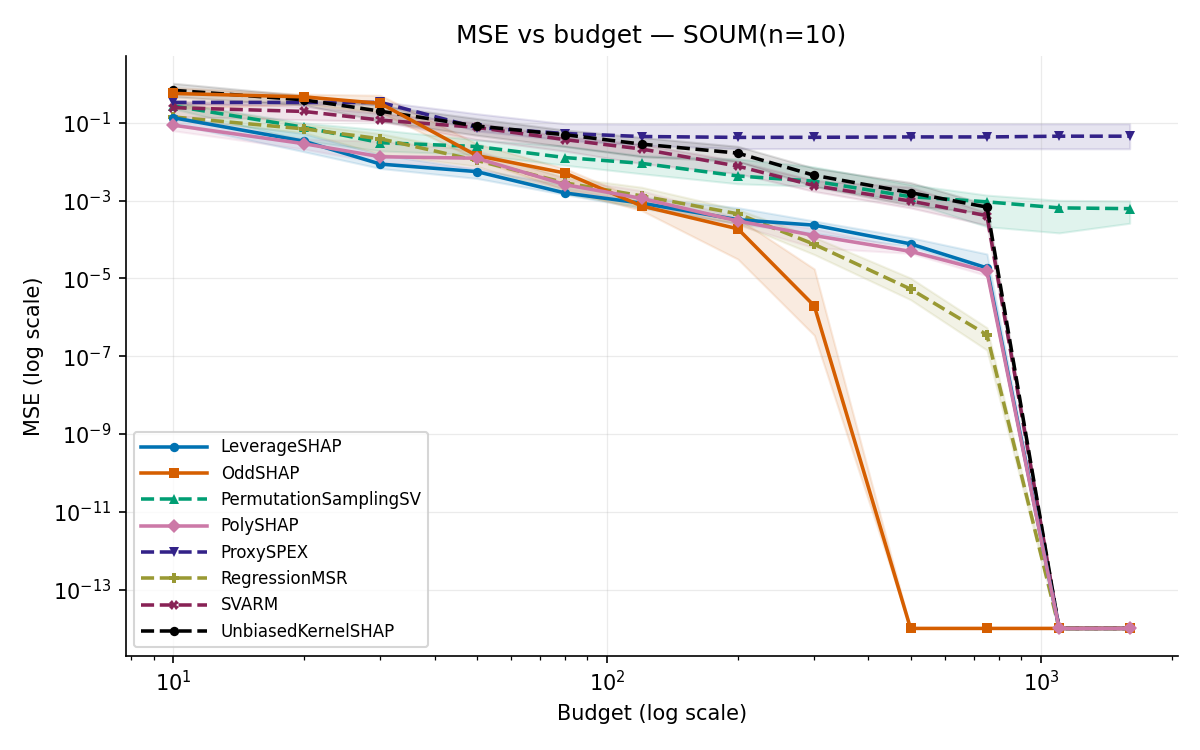
\includegraphics[width=\textwidth]{figures/bench-soum-n10.png}
    \caption[MSE against budget on SOUM ($n=10$)]{MSE against budget on SOUM ($n=10$), a small
        game. Every method falls to the numerical floor as the budget approaches full enumeration
        ($2^{10} = 1024$); $24\%$ of all small-game results are exact in this sense. Ranks in that
        region are tie-breaking rather than comparison, which is why the aggregate over all eleven
        games should not be read as a verdict.}
    \label{fig:benchmark:soum}
\end{figure}

\paragraph{Threats to validity.}
The value function is not any paper's, so this chapter compares the methods with each other and
does not test any paper's claim; that is what Chapters~\ref{sec:oddshap}--\ref{sec:polyshap} are
for. Coverage is uneven, and average ranks across methods that ran in different numbers of cells
are not directly comparable, because a method that declines a budget is scored only where it ran.
\oddshap{} declines 50 cells, all at $m = d$ or $2d$ on the four smallest games, where the budget
falls below its minimum of $\eta = 10$ evaluations; it declines none on the large games, where it
ran in all 480. SPEX declines 680 cells and ProxySPEX 10. ShaplEIG is registered but needs an
optional extra that was not installed, so it is skipped in all 1{,}320 of its cells and appears in
no figure. Ten predictions per game make the quartiles a coarse envelope rather than a confidence
interval. Finally, FourierSHAP and the fixed-budget FFD variants belong to
\citet{Fumagalli.2026}'s own comparison but are not implemented in \shapiq{}, so the baselines
here are that paper's set intersected with what was available, not the set in full.
